% themenbereiche
%Geometrische simpliziale Komplexe; Triangulierungen; abstrakte
%simpliziale Komplexe; Beispiele simplizialer Komplexe


%homotopiegruppen sind invarianten von top räumen, einfaches kriterium
%zur unterscheidung von top räumen


% schlagwort verzeichnis
%TODO: folgende begriffe müssen definiert, verwendet und verstanden sein: simplex, seite, eckmenge, dimension, simplizialkomplex, n-skelett, geometrischer simplizialkomplex, geometrische realisierung, schwache topologie, triangulierbar, simpliziale abbildung, baryzentrische koordinaten, 

%warum simpliziale komplexe bzw mengen gebraucht werden, selbe homotophietheorie und selbe homotopiegruppen, einfachere berechnung der homotopiegruppen.

\section{Geometrische Simpliziale}

Simpliziale sind rein kombinatorische Objekte, mit denen man auf gute
Art und Weise topologische Räume beschreiben kann, insbesondere ihre
Homologiegruppen berechnen kann.

Wir definieren zunächst grundlegende Begriffe für die spätere
Defintione der Simpliziale.
\begin{Def}[Geometrisch unabhängig\footnote{Oder auch affine
    Unabhängigkeit}]
  \label{def:1}
  Eine endliche Menge $\{ a_0\ldots a_n \} \subset \R^N$ heißt
  \textbf{geometrisch unabhängig}, falls das System von Vektoren
  \begin{gather*}
    a_0 - a_1 , \ldots , a_0 - a_n
  \end{gather*}
  unabhängig im Sinne der Linearen Algebra ist. Eine beliebige Menge
  $A \subset \R^J$ ist geometrisch unabhängig, falls jede endliche
  Teilmenge von $A$ geometrisch unabhängig im obigen Sinne.
\end{Def}

Zeige für spätere Verwendung eine äquivalente Formulierung der
geometrischen Unabhängigkeit.

\begin{Lem}\label{lem:1}
  Teilsysteme von geometrisch unabhängigen Systemen sind geometrisch
  unabhängig. Eine endliche, geometrische unabhängige Menge vom $\R^N$
  hat maximal $N+1$ Elemente und für ein Menge
  $\{ a_0 , \ldots , a_n \} \subset \R^N$ sind folgende Aussagen
  zueinander äquivalent:
  \begin{enumerate}[$(i)$]
  \item $\{ a_0 , \ldots , a_n \}$ ist geometrisch unabhängig
  \item Für $\sum\limits_{i=0}^n t_i = 0$ und
    $\sum\limits_{i=0}^n t_i a_i = 0$ folgt stets $t_i = 0$ für alle
    $i \in \{ 0,\ldots,n\}$
  \end{enumerate}
  \begin{proof}
    Sei $\{ a_0 , \ldots , a_n \}$ ein geometrisch unabhängiges System
    und hierzu ein Teilsystem $\{ a_{i_0},\ldots,a_{i_r} \}$.  Sei
    \OE~ $i_0 = 0$ , sonst nummeriere um oder betrachte ein anderes
    $i_j$, so dass für dieses $i_j$ das ursprüngliche geometrisch
    unabhängige System der Punkt $a_{i_j}$ als Basispunkt gewählt
    werden kann. Nun ist nach \cref{def:1},
    $ a_0 - a_1 , \ldots , a_0 - a_n$ linear unabhängig und somit auch
    das Teilsystem $ a_0 - a_ {i_1}, \ldots , a_0 - a_{i_r}$.  Sei nun
    $A \subset \R^N$ ein endliches, geometrisch unabhängig System,
    dann ist nach \cref{def:1}, für ein Element $a \in A$, das System
    $\set{ a - a'}{a' \in A \setminus \sset{a} }$ linear unabhängig.
    Die Kardinalität des Systems ist offentsichtlich durch die
    Dimension des Vektorraum beschränkt und somit maximal gleich
    $N+1$. Für den letzten Teil des Beweises nutze man folgende
    Äquivalenzen
 % \newcommand{\lla}{~\Leftrightarrow~}
 %    \begin{align*}
 %      \forall~t_i =0 
 %      \overset{(1)}{\lla}
 %      &\sum\limits_{i=1}^n t_i(a_o - a_i) = 0\\
 %      \lla
 %      &\sum\limits_{i=1}^n t_i a_i = a_0 \cdot \sum\limits_{i=1}^n t_i\\
 %      \overset{(2)}{\lla}
 %      &\sum\limits_{i=1}^n t_i a_i = - a_0 t_0\\
 %      \lla
 %      &\sum\limits_{i=0}^n t_i a_i = 0
 %    \end{align*}
 %    Hierbei steht $(1)$ für die Aussage $$
    \begin{description}
    \item[$ii)
      \Rightarrow i)$] Seien $\sp{0}{n} t_i = 0$ und $\sp{0}{n} t_i
      a_i = 0$, dann folgt 
      \begin{gather*}
        0 = \sp{0}{n} t_i a_i = t_0 a_0 + \sp{1}{n} t_i a_i = -a_0
        \sp{1}{n} t_i + \sp{1}{n} t_i a_i = \sp{1}{n} t_i (a_i - a_0)
    \end{gather*}
    und somit $t_i = 0$ für alle $i$.
      \item[$ii) \Rightarrow i)$]
        Sei nun $\sp{1}{n} t_i (a_i - a_0) = 0$ 
%TODO: noch nicht verstanden        
    \end{description}
  \end{proof}
\end{Lem}

In der nächsten Definition wird das in diesem Vortrag zugrundeliegende
Objekt von Interesse definiert. Dieses dient im weiteren Verlauf als
Baustein für Komplexe.

\begin{Def}[geometrischer $n$-Simplex]
  Zu einem geometrisch unabhängigen System \gs $\subset \R^N$, nennt
  man die Menge
  \begin{gather*}
    \set{\sum\limits_{i=0}^n t_i a_i \in \R^N}{ t_i \in [0,1] ~,~
      \sum\limits_{i=0}^n t_i = 1}
  \end{gather*}
  den (geometrischen) $n$-Simplex und schreibt $a_0 \ldots a_n$ oder
  ohne die Punkte genauer zu spezifizieren $\sigma^n$ mit $n$ die
  Dimension des geometrischen Systems. Dies ist die Menge aller
  Konvexkombinationen des Systems \gs. Als Konvention ist der Simplex
  stets in den $\R^N$ eingebettet für ein $N \geq n$.
\end{Def}


% TODO: erstes Beispiel zu einem simplex, zeiche in tikz \sigma^k für
% k =0,1,2,3
\begin{Bsp}[Einfache Beispiele]
Definiere den Standardsimplex $\sigma^n \coloneqq e_0\ldots e_n$. Die Fälle $n = 0,1,2,3$ sind hier aufgezeichnet
\newline

%{$n=0$}\hfill{$n=1$}\hfill{$n=2$}\hfill{$n=3$}

% objekte müssen nebeneinander sein

% 0 - simplex, punkt
% besseren punkt ausdenken, kleinen kreis mit blauer farbe, 
\begin{tikzpicture}
  \node (s) at (0,2) {$n=0$};
  \fill (0,0) circle[radius=0.07cm];
\end{tikzpicture}
\hfill
%1 - simplex, gerade
\begin{tikzpicture}
 \node (s) at (0,2) {$n=1$};
  \fill (-0.7,0) circle[radius=0.07cm];
%  \draw[thin] (0,0)--++(1,0);
  \fill (0.7,0) circle[radius=0.07cm];

  \draw [thin,fill=lightgray] (-0.7,0) to (0.7,0) to (-0.7,0);
\end{tikzpicture}
\hfill
%2 - simplex, gleichseitiges dreieck
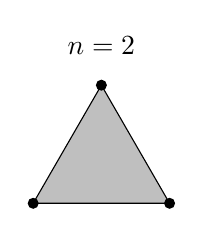
\begin{tikzpicture}
    \node (s) at (0,1.5) {$n=2$};
  \draw [thin,fill=lightgray] (90:1) to (210:1) to (330:1) to (90:1);
    \fill (90:1) circle[radius=0.07cm];
    \fill (210:1) circle[radius=0.07cm];
    \fill (330:1) circle[radius=0.07cm];
\end{tikzpicture}
\hfill
%3 - simplex, tetraeder
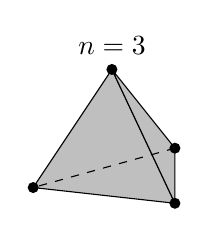
\begin{tikzpicture}
  \node (s) at (1,2) {$n=3$};
\draw [thin,fill=lightgray] (0,0.2) to (1.8,0) to (1,1.7) to (0,0.2);
\draw [thin,fill=lightgray] (1.8,0) to (1.8,0.7) to (1,1.7) to (1.8,0);
\draw [thin,dashed] (1.8,0.7) to (0,0.2);

    \fill (0,0.2) circle[radius=0.07cm];
    \fill (1.8,0) circle[radius=0.07cm];
    \fill (1,1.7) circle[radius=0.07cm];
    \fill (1.8,0.7) circle[radius=0.07cm];
\end{tikzpicture}

\end{Bsp}

Um die Punkte innerhalb eines Simplexes unabhängig von der Lage im
umliegenden Raum zu beschreiben sind spezielle Koordinaten
vonnöten. Diese werden nun definiert und ihre Eindeutigkeit und
Stetigkeit bezüglich des Punktes bewiesen.


\begin{Lem}[Baryzentrische Koordinaten]\label{lem:bary}
  \normalfont Es bezeichnet $x$ einen Punkt aus dem Simplex
  $\sigma^n = a_0\ldots a_n$. In der Darstellung
  $x = \sum_{i=0}^n t_i a_i$ nennt man $t_i$ \textbf{baryzentrische}
  Koordinaten. Diese sind durch $x$ eindeutig bestimmt und als
  Funktionen $t_i : \sigma^n \subset \R^N \rightarrow [0,1]$ stetig.
  \begin{proof}
    Beweise zunächst die Eindeutigkeit über die äquivalente
    Formulierung der geometrischen Unabhängigkeit aus \cref{lem:1}
    \begin{description}
    \item[Eindeutigkeit: ] Seien zwei Darstellungen
      \begin{gather*}
        x = \sum\limits_{i=0}^n t_i a_i = \sum\limits_{i=0}^n s_i a_i
        \text{ mit } \sum\limits_{i=0}^n t_i = \sum\limits_{i=0}^n s_i
        = 1
      \end{gather*}
      gegeben, so folgt durch umformen
      \begin{gather*}
        \sum\limits_{i=0}^n (t_i - s_i ) \cdot a_i = 0 \text{ und }
        \sum\limits_{i=0}^n t_i - s_i = 0.
      \end{gather*}
      Da $\sset{a_0 , \ldots , a_n}$ ein geometrisch unabhängiges
      System ist, folgt durch \cref{lem:1} das
      $t_i - s_i = 0 \Leftrightarrow t_i = s_i$, also die Koordinaten
      eindeutig sind.
    \item[Stetigkeit: ] Aufgrund der Eindeutigkeit der baryzentrischen
      Koordinaten sind die Abbildungen $t_i (x)$ wohldefiniert.
      Definiere die Vektoren $b_i \coloneqq a_i - a_0$ und erweitere
      das linear unabhängige System $\set{ b_i }{ 1 \leq i \leq n}$ zu
      einer Basis vom $\R^N$. Schreibe hierfür $\set{ b_i
      }{ 0 \leq i \leq N}$. Betrachte nun die Differenz $x - a_0$
%	TODO: auf diegleichung mit cref referenzieren
      \begin{align*}
        x - a_0 &= \sp{0}{n} t_i a_i - 1 \cdot a_0\\
                &\overset{(*)}{=} \sp{0}{n} t_i a_i - \sp{0}{n} t_i a_0\\
                &= \sp{1}{n} t_i \cdot (a_i - a_0)\\
                &= \sp{1}{n} t_i b_i\\
                &= \sp{1}{n} t_i b_i + \sp{n+1}{N} 0 \cdot b_i
      \end{align*}
      Hierbei entspricht $(*):$ $\sp{0}{n} t_i = 1$. Schreibe dies nun als
      ein lineares Gleichungssystem, mit
      $x=(x_1,\ldots,x_N),a_i=(a_i^1,\ldots,a_i^N),t=(t_1,\ldots,t_n,0,\ldots,0),B=(b_i^j)_{i,j}$,
      so schreibt sich die obige Gleichung wie folgt:
      $x-a_0 = B\cdot t$. Durch umformen nach $t$, also dem
      invertieren der Matrix $B$, wird ersichtlich weshalb die $t_i(x)$
      für $1 \leq i \leq n$ stetige Funktionen sind. Mit
      $t_0 = 1 - \sp{1}{n} t_i$ ist die Behauptung gezeigt.
      % BEMERKUNG: dies zeigt auch die eindeutigkeit der t_i, da
      % lineares gleichungssystem, eindeutige lösung
    \end{description}
  \end{proof}
\end{Lem}

Eine weitere Definition

\begin{Def}[Eckmenge, Dimension, Seite, Rand, Inneres]
  Sei $\sigma = a_0 \ldots a_n$ ein geometrischer $n$-Simplex, so
  definiere folgende geometrische Objekte
%TODO: soll die nummerierung fett gehalten sein
  \begin{enumerate}[\textbullet]%{\bfseries1)}]
  \item Die Menge $\{ a_0 , \ldots , a_n \}$ bezeichnet man als
    \textbf{Eckmenge} $\V(\sigma)$ von $\sigma$.
  \item Ein Teilmenge $\tau \subset \sigma$ heißt \textbf{Seite} falls
    $\tau$ einen Simplex bildet. Eine Seite heißt \textbf{echt} falls
    sie von $\sigma$ verschieden ist.
	\item Die \textbf{Dimension} von $\sigma$ ist die Zahl $n$ bzw. 
		$\dim(\sigma) = \gr{\V(\sigma)} - 1$
  \item Der \textbf{Rand} von $\sigma$ ist die folgende Menge:
    \begin{gather*}
      \partial\sigma = \bigcup \; \left\{ \tau \; \Big| \; \tau \text{
          ist echte Seite von } \sigma \right\}
    \end{gather*}
  \item Das \textbf{Innere} des Simplex ist die Menge
    \begin{gather*}
    	\Int(\sigma) \coloneqq \sigma \setminus \partial\sigma
    \end{gather*}
  \end{enumerate}
\end{Def}

Zur vorherigen Definition ein anschauliches Beispiel.

\begin{Bsp}
  Betrachte den Simplex $\sigma^2 = e_0e_1e_2$.
\newline

%TODO: if possible, position with parbox
\centering
\parbox{0.7\linewidth}{% 
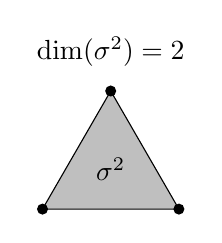
\begin{tikzpicture}
    \node (s) at (0,1.5) {$\dim(\sigma^2)=2$};

  \draw [thin,fill=lightgray] (90:1) to (210:1) to (330:1) to (90:1);
    \node (title) at (0,0) {$\sigma^2$};
    \fill (90:1) circle[radius=0.07cm];
    \fill (210:1) circle[radius=0.07cm];
    \fill (330:1) circle[radius=0.07cm];
\end{tikzpicture}
\hfill
\raisebox{0.8cm}{$=$}
\hfill
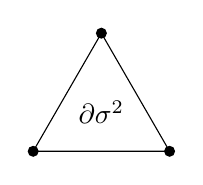
\begin{tikzpicture}
  \draw [thin] (90:1) to (210:1) to (330:1) to (90:1);
    \node (title) at (0,0) {$\partial\sigma^2$};
    \fill (90:1) circle[radius=0.07cm];
    \fill (210:1) circle[radius=0.07cm];
    \fill (330:1) circle[radius=0.07cm];

\end{tikzpicture}
\hfill
\raisebox{0.8cm}{$\cup$}
\hfill
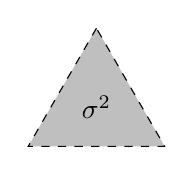
\begin{tikzpicture}
  \draw [dashed,fill=lightgray] (90:1) to (210:1) to (330:1) to (90:1);
    \node (title) at (0,0) {$\Int\sigma^2$};
\end{tikzpicture}
}
\end{Bsp}
% TODO: tikz bilder einfügen von beispielen in denen für ein beispiel symbolisch die obrigen definitionen angegeben werden

Es werden nun einige Charakterisierungen und Aussagen über die
Simplizes und deren geometrischen Objekten bewiesen.

\begin{Satz}
  \normalfont Sei $\sigma = a_0 \ldots a_n $ ein $n$-Simplex,
  $x \in \sigma$ mit der baryzentrischen Darstellung
  $x=\sum\limits_{i=0}^n t_i a_i$ , so gelten folgende Aussagen:
  \begin{enumerate}[$(a)$]
  \item
    $x \in \partial\sigma \Leftrightarrow \exists \; 0 \leq i \leq n :
    t_i = 0$
  \item \label{satz:a}
    $x \in \Int(\sigma) \Leftrightarrow \forall \; 0 \leq i \leq n :
    t_i > 0$
  \item Jeder Simplex $\sigma$ ist eine konvexe, kompakte Teilmenge (
    vom $\R^N$), insbesondere ist die konvexe Hülle von
    $\{ a_0 \ldots a_n \}$ identisch mit dem Simplex $\sigma$.
  \item Das Innere $\Int(\sigma)$ ist offen und konvex.
  \item Zwei Simplexe der selben Dimension sind homöomorph.
  \item Es gilt $\overline{\Int(\sigma)} = \sigma$.
  \item Es gibt einen Homöomorphismus $\sigma \simeq \Bn$, der das
    Innere $\Int(\sigma)$ auf die $\Sp^{n-1}$ abbildet.
  \end{enumerate}
  \begin{proof}
    \begin{enumerate}[$a)$:]
      % a)
    \item
      \begin{description}
      \item[\glqq $\Rightarrow$\grqq] Sei $x$ im Rand
        $\partial\sigma$, so liegt der Punkt in einer echten Seite
        $\tau$ von $\sigma$. Sei \OE~ $\tau = a_0 \ldots a_m$ für ein
        $m < n$. Dann hat $x$ eine eindeutige baryzentrische
        Darstellung bezüglich des Simplex $\sigma$, aber auch eine
        eindeutige Darstellung bezüglich der Seite $\tau$, also
        existieren $t_i,s_i$, mit
        \begin{gather*}
          x = \sp{0}{m} s_i a_i = \sp{0}{n} t_i a_i .
        \end{gather*}
        Durch die Eindeutigkeit der Darstellung folgt unmittelbar das
        ein $0 \leq i \leq n$ existieren muss, so dass $t_i = 0$ gilt.
      \item[\glqq $\Leftarrow$ \grqq] Gilt nun umgekehrt $t_i = 0$ für
        ein $0 \leq i \leq n$, liegt der Punkt $x$ in der echten Seite
        $a_0 \ldots a_{i-1} a_{i+1} \ldots a_n$ und damit im Rand.
      \end{description}

      % b)
    \item Diese Aussage folgt unmittelbar als Negation von a) und der
      Tatsache das $\sigma = \partial\sigma \cup \Int(\sigma)$ eine
      disjunkte Vereinigung ist.

      % c)
    \item 
      \begin{description}
      \item[kompakt:] Definiere eine stetige Abbildung
        $f : \R^{n+1} \rightarrow \R^N$ mit
        $ f(t_0,\ldots ,t_n) = \sp{0}{n} t_i a_i$, diese ist stetig da
        nach \cref{lem:bary} die baryzentrischen Koordinaten es
        sind. Die Menge
        \begin{gather*}
          A= \set{ (t_0,\ldots,t_n) \in \R^{n+1}}{ \sp{0}{n} t_i = 1
            \text{ und für alle } i , t_i > 0}
        \end{gather*}
        ist kompakt, da man sie durch die $1$-Norm $\nn_1$ wie folgt
        schreiben kann $A = (\nn_1)^{-1}(\{ 1 \}) \cap
        [0,1]^{n+1}$.
        Somit ist $\sigma = f(A)$ als Bild einer kompakten Mengen
        unter einer stetigen Abbildung wieder kompakt.
      \item[konvex:] Seien zwei Punkte $x,y \in \sigma$ gegeben und
        ihre baryzentrischen Darstellungen seien $x = \sum t_i a_i$,
        $y = \sum s_i a_i$ mit $\sum t_i = \sum s_i = 1$. Dann folgt
        für eine Konvexkombination mit $\lambda \in [0,1]$
        % TODO nur die zweite gleichung darf eine beschriftung tragen
        \renewcommand*{\theequation}{$*$}
        \begin{align}
          \nonumber
          \lambda x + (1- \lambda)y &= \lambda \cdot \sp{0}{n} t_i a_i%
                                      + (1-\lambda) \cdot \sp{0}{n} s_i a_i \\
                                    &= \sp{0}{n} (\lambda t_i +%
                                      (1-\lambda) s_i) \cdot a_i  
        \end{align}
        Jeder Punkt dieses Verbindungsstück von $x$ und $y$ liegt
        wieder in $\sigma$, denn
        \begin{align*}
          \sp{0}{n} \lambda t_i + (1-\lambda) s_i 
          &= \lambda \cdot \sp{0}{n} t_i + (1-\lambda) \cdot \sp{0}{n} s_i \\
          &= \lambda + (1 - \lambda) = 1
        \end{align*}
        Also folgt $\lambda x + (1- \lambda)y \in \sigma$.  

      \item[Konvexe Hülle:] Es ist zu zeigen
        $\conv(\sset{a_0,\ldots , a_n}) = \sigma$, hierbei gilt
        $\sset{a_0,\ldots,a_n} \subset \sigma$, da $\conv$ monoton
        ist, also $\conv(\sset{a_0,\ldots , a_n}) \subset \sigma$.
        
        Nun gilt $a_ia_j \subset \conv( \sset{a_0,\ldots , a_n} )$, da
        mit $a_i \in \ch$ auch jeder Punkt der sich als
        Konvexkombinationen schreiben lässt in der konvexen Hülle
        liegt. Durch Induktion über $n$, folgt nun mit der Darstellung
        $x = t_0 a_0 + \lambda \cdot \sp{1}{n} \frac{t_i}{\lambda}
        a_0$ die andere Inklusion.
        
    %     Beweise zunächst folgende Darstellung
    %   \begin{gather*}
    %     \sigma = \bigcup \set{ a_0 b}{b \in a_1\ldots a_n}
    %   \end{gather*}
    %   Betrachte hierzu für einen Punkt $a_0 \not= x \in \sigma$ dessen baryzentrische
    %   Darstellung, so folgt
    %   \begin{align*}
    %     x &= \sp{0}{n} t_i a_i \\
    %       &= t_0 a_0 + \sp{1}{n} t_i a_i \\
    %       &= t_0 a_0 + \lambda \cdot \sp{1}{n} \frac{t_i}{\lambda} a_i 
    %   \end{align*}
    %   Mit $\lambda \coloneqq \sp{1}{n} t_i \not= 0$, so ist
    %   $ \sp{1}{n} \frac{t_i}{\lambda} a_i \in a_1 \ldots a_n$, denn
    %   $\sp{1}{n} \frac{t_i}{\lambda} = \frac{1}{\lambda} \cdot
    %   \sp{1}{n} t_i = 1$.
      
    %   % konvex durch andere darstellung und kompaktheit durch bild der
    %   % abbildung von t_0 ... t_n auf \sum t_i a_i , kompaktes bild
    %   % TODO: beweis für kompaktheit und konvex, nutze affine
    %   % transformation für obda \sigma ist e_0 ... e_n nutze basis,
    %   % und t_i sind beschränkt
     \end{description}

     % d)
   \item \begin{description}
     \item[offen:] Da jede Seite $\tau \subset \sigma$ wieder ein
       Simplex ist, ist diese auch kompakt, insbesondere
       abgeschlossen. Nun ist der Rand $\partial\sigma$ Vereinigung
       dieser abgeschlossen Mengen, also wieder abgeschlossen. Das
       Innere ist nun das Komplement der abgeschlossen Menge, also
       offen.
     \item[konvex:] Seien zwei Punkte $x,y \in \Int(\sigma)$ gegeben,
       dann
       % TODO: besseren cref verwenden
       gilt nach \cref{satz:a} , das für die baryzentrischen
       Koordinaten der Punkte~~$t_i,s_i >0$ gilt. Sei nun
       $\lambda \in [0,1]$, so gilt für die baryzentrischen
       Koordinaten der Konvexkombinationen $\lambda x + (1-\lambda y)$
       die Darstellung $\lambda t_i + (1-\lambda)s_i$. Dies ist stets
       größer als $0$.
        \end{description}
      \item Zeige das ein beliebiger Simplex $\sigma^n$ homöomorph zum
        Standardsimplex $e_0\ldots e_n$ ist. Betrachte hierfür die
        affine Transformation $f(x) = Ax+b$ mit $A \in \GL(N,\R)$ und
        $b \in \R^N$, die $a_i$ auf $e_i$ abbildet. Dies ist
        offentsichlich ein Homöomorphismus.
      \item Da $\sigma$ abgeschlossen ist und
        $\overline{\hspace{0.1cm} \cdot \hspace{0.1cm}}$ ist monoton
        gilt: $\overline{\Int(\sigma)} \subset \sigma$.

        Sei nun $x \in \sigma$. Nutze die disjunkte Zerlegung des
        Simplex $\sigma = \partial\sigma \cup \Int(\sigma)$. Dann
        unterscheide die beiden Fälle das $x$ in genau einem der
        beiden Mengen liegt. Für
        $x \in \Int(\sigma) \subset \overline{\Int(\sigma)}$ sind wir
        schon fertig. Für $x \in \partial\sigma$ nutze die
        Charakterisierung der Elemente des Randes, also
        $x \in \partial A \Leftrightarrow \forall U \text{ offene
          Umgebung von } x : U \cap A \not= \emptyset \text{ und } U
        \cap A^c \not= \emptyset $.
        Und mithilfe der Charakterisierung der Elemente des
        Abschlusses:
        $ x \in \overline{A} \Leftrightarrow \forall U \text{ offene
          Umgebung von }x : U \cap A \not= \emptyset$.
        Und somit folgt die Behauptung.

        % g)
    \item Betrachte die stetige Abbildung
      $f : \R^{n+1} \setminus \sset{0} \rightarrow \Sp^n, f(x) = \frac{x}{\nn[x]}$.
      Definiere für $a \in \Int(\sigma), p \in \R^N \setminus \{ 0 \}$ die Menge
      $ap_+ \coloneqq \set{ a + tp}{ t \geq 0}$. Dann beweise folgende Behauptung.
      \begin{Beh}
        Der Schnitt $\partial\sigma \cap ap_+$ hat genau ein Element.
        \begin{proof}
          Zur Existenz des Element betrachte die Menge
          $ap_+ \cap \Int(\sigma)$.  Diese ist homöomorph zu $[0,b)$
          für ein $b>0$ und somit existiert bezüglich des
          Homöomorphismus durch den Punkt $b$ ein Schnittpunkt der
          Halbgerade mit dem Rand.
          
          Seien nun zwei Punkte $x,y \in \partial\sigma$ die auch in
          $ap_+$ enthalten sind. Seien $t_x, t_y \in \R_{> 0}$ die
          Paramter, so dass gilt: $a + t_i \cdot p = i$ mit
          $i \in \sset{x,y}$ und sei \OE~ $t_y < t_x$. Dann folgt
          durch umformen
          \begin{gather*}
            x = (1-t) a + ty \text{ mit } t=\frac{t_y}{t_x} < 1
          \end{gather*}
          Wähle nun eine Folge $\sset{y_n} \subset \Int(\sigma)$ die
          gegen $y$ konvergiert und setze
          $a_n \coloneqq \frac{x -ty_n}{1-t}$. Dann konvergiert nach
          Konstruktion $a_n$ gegen $a$ und da $a \in \Int(\sigma)$ in
          einer offenen Menge enthalten ist, existiert ein $n \geq 0$
          so dass für alle $m \geq n$ gilt $a_m \in \Int(\sigma)$. Somit
          liegt nun $x = (1-t) a_n + ty_n$ in $\Int(\sigma)$ da die
          Menge konvex ist und die Folgenglieder ab einem $m$ in der
          Menge $\Int(\sigma)$ liegen, dies ist ein Widerspruch zu
          $x \in \partial\sigma$.
        \end{proof}
      \end{Beh}
      Sei nun \OE~ $0 \in \sigma$, sonst wende Translation auf
      $\sigma$ an.  Schränke nun die Abbildung $f$ auf die Menge
      $\partial\sigma$ ein. Nach obiger Behauptung ist die Abbildung
      $f_{| \partial\sigma} : \partial\sigma \rightarrow \Sp^n$
      bijektiv und stetig. Da $\partial\sigma$ und $\Sp^n$ kompakt und
      hausdorffsch sind ist die Abbildung auch ein Homöomorphismus.
      
      Setze nun als Umkehrabbildung $g : \Sp^n \rightarrow \partial\sigma$ 
      und erweitere diese zu einem Homöomorphismus der Form
      \begin{gather*}
        G : \Bn \rightarrow \sigma , \hspace{0.5cm}
        x \mapsto 
        \begin{cases}
          0 & , x = 0 \\
          \nn[g(\frac{x}{\nn[x]})] \cdot x & \text{, sonst}
        \end{cases}
      \end{gather*}
      Diese Abbildung erfüllt die gewünschten Eigenschaften.
    \end{enumerate}
  \end{proof}
\end{Satz}


\begin{Bem}
  Für eine beliebige Menge $J$ ist der Raum der Funktionen $\R^J$ ein
  $\R$-Vektorraum, dessen Elemente als Tupel $(x_j)_{j \in J}$
  geschrieben werden. Betrachte den Untervektorraum
  $\E^J \coloneqq \bigoplus\limits_{j \in J} \R$ der Elemente die bis
  auf endlich viele von Null verschieden sind. Definiere für zwei
  Elemente $x,y \in \E^J$ eine Metrik
  \begin{gather*}
    \gr{x-y} \coloneqq \sup \set{ \gr{x_j - y_j } }{ j \in J}.
  \end{gather*}
  Die obigen Definitionen und Aussagen funktionieren ebenso falls man
  die Simpliziale indem Raum $\E^J$ betrachtet, somit ist sind 
  auch geometrische Simpliziale der Kardinalität größer als der von $\R$
  möglich.
\end{Bem}




%%% Local Variables:
%%% mode: latex
%%% TeX-master: "main"
%%% End:
